% metadata_file.tex - An article describing the metadata file format used as annotation for libraries in the AltLab Translocation Pipeline.

\documentclass{article}
%\usepackage{times}
\usepackage{graphicx}
\usepackage{float}
\DeclareGraphicsExtensions{.pdf}
\usepackage[labelfont=bf,labelsep=period]{caption}
\usepackage[colorlinks=true, urlcolor=blue]{hyperref}



\begin{document}

\title{Metadata File Specification \\ \large Format and Content of the Annotation File for Libraries to be Analyzed with the Translocation Pipeline}
\author{Robin M. Meyers\\
  Laboratory of Fredrick W. Alt,\\
  Boston Children's Hopsital, Harvard Medical School\\
  \href{mailto:robin.meyers@childrens.harvard.edu}{\texttt{robin.meyers@childrens.harvard.edu}}}
\date{Created: January 15, 2014; Updated: \today}
\maketitle

\begin{abstract}
Guidelines for creating a metadata file are presented. The metadata file delivers important details to the pipeline software about the translocation library and its preparation and analysis. Each record in the metadata file specifies a single library.
\end{abstract}

\section{Introduction}
\paragraph{}
The purpose of the metadata file is to to deliver important details about the translocation library to the pipeline software so that it can be analyzed correctly. It was designed to include as little extraneous information as possible, while still allowing flexibility to account for the diversity of library types that the lab generates. Each record in the metadata file annotates a single library and must be created according to the following guidelines as strictly as possible to ensure consistency between libraries.

\section{The Metadata File}
\paragraph{} The metadata file is a data table that contains a header row, followed by a row for each library. There is no limit to the number of libraries listed in the file. Each column contains a field specifying a property about each library. It is appropriate for researchers to create and edit this file as a Microsoft Excel spreadsheet and save it as either an ``Excel Workbook'' (*.xlsx/xls) or a ``Tab Delimited Text'' (*.txt) from the ``Format'' drop-down menu in the ``Save As...'' dialogue box.  

\subsection*{Columns}
\paragraph{} The header row conisists of the names of the columns. Although there is no strict ordering of the columns, it is recommended that the order below is used for consistency. Please refer to the following sections for a more detailed description of each field.
\begin{itemize}
  \item \textbf{Library} - name of the library, typically the researcher's initials followed by a three digit, zero-padded number (\emph{e.g.} \texttt{AB001})
  \item \textbf{Sequencing} - name of the sequencing run, typically ``Alt'' followed by a three digit, zero-padded number(\emph{e.g.} \texttt{Alt001})
  \item \textbf{Researcher} - the researcher's name
  \item \textbf{Assembly} - the genome build to be aligned against (\emph{e.g.}) \emph{mm9} or \emph{hg19})
  \item \textbf{Chr} - name of the chromosome harboring the breaksite locus/cassette
  \item \textbf{Start} - start coordinate of the breaksite locus/cassette
  \item \textbf{End} - end coordinate of the breaksite locus/cassette
  \item \textbf{Strand} - breaksite locus/cassette orientation, either ``\texttt{+}'' or ``\texttt{-}''
  \item \textbf{Breakseq} - breaksite cassette sequence \emph{(non-endogenous breaksite libraries only)}
  \item \textbf{Breaksite} - targeted site coordinate with respect to \texttt{Breakseq}  \emph{(non-endogenous breaksite libraries only)}
  \item \textbf{MID} - multiplex identifier sequence
  \item \textbf{Primer} - primer sequence
  \item \textbf{Adapter} - adapter sequence
  \item \textbf{Cutter} - frequent cutter sequence, if applicable
  \item \textbf{Description} - an optional description of the library (\emph{e.g.} genotype background, breaksite strategy, etc)
\end{itemize}

\section{Identifier Fields}
\textbf{Library, Sequencing, Researcher, Assembly, Description}
\paragraph{} The identifier fields are all fairly straight forward and do not require much further explanation. It is recommended that the researcher is consistent with \texttt{Library}, \texttt{Sequencing}, and \texttt{Researcher} names although they will not affect pipeline operation except for the naming of the files. The \texttt{Description} field is used only for documentation and is optional. It cannot include any newlines, carriage-returns, or any special characters. The \texttt{Assembly} field specifies the genome build to be used as the alignment reference.

\section{Annotating the Breaksite}
\textbf{Chr, Start, End, Strand, Breakseq, Breaksite}
\paragraph{} There are two major types of translocation libraries that the Alt Lab currently produces, characterized by either an endogenous breaksite locus or non-endogenous breaksite cassette (\emph{i.e.} an I-SceI cassette). The pipeline was engineered to handle these two cases as similarly as possible, and is described fully in the pipeline documentation. However, the interpretation of some columns in the metadata file is different for each library type.

\subsection{Endogenous Breaksite Libraries}
\begin{figure}[H]
\centering
  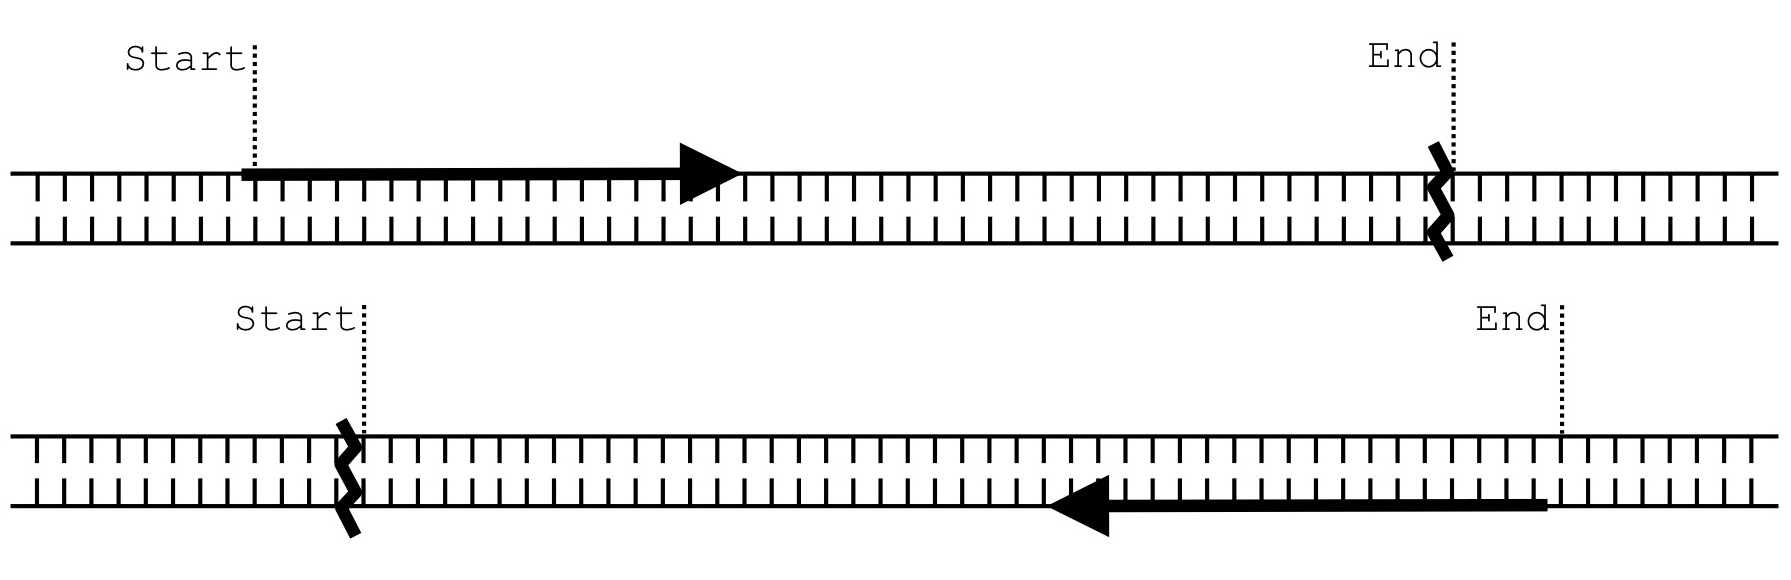
\includegraphics[width=\textwidth]{endogenous_breaksite}
\caption{\textbf{Endogenous breaksite} strategies are shown in the ``\texttt{+}'' strand orientation \textbf{(Top)} and ``\texttt{-}'' orientation \textbf{(Bottom)}. Diagrams are oriented so that chromosomal coordinates increase from left to right. The bold arrow represents the priming site and the jagged line represents the targeted nuclease site. The appropriate \texttt{Start} and \texttt{End} coordinates are marked. }
\label{overflow}
\end{figure}
\paragraph{} For endogenous breaksite libraries, the breaksite is fully annotated simply by specifying the priming site and targeted nuclease site. To do this, the metadata file needs only to use the \texttt{Chr}, \texttt{Start}, \texttt{End}, and \texttt{Strand} fields. The \textbf{breaksite locus} is defined as the region from, and including, the first (5') basepair of the priming site to the targeted site, which should in theory occur between two basepairs. \emph{Note: For targeted sites with overhangs, there is a unique site on either strand. It is recommended to maintain a convention of either selecting the targeted site that occurs farthest from the priming site or selecting the targeted site on the same strand as the primer.} The \texttt{Chr} is the name of the chromosome that contains the breaksite locus (\emph{e.g.} \texttt{chr15}). The \texttt{Strand} is the orientation of the breaksite locus on the chromosome in the primer-to-target direction, either ``\texttt{+}'' or ``\texttt{-}''. In the ``\texttt{+}'' orientation, the primer aligns to the ``\texttt{+}'' strand and the priming site occurs before the targeted site in order of chromosomal coordinates. The reverse is true for a breaksite locus in the ``\texttt{-}'' orientation. The pipeline follows the genomic annotation convention of requiring the start coordinate of an annotated region to not be greater than the end coordinate, regardless of the orientation of the annotation. Therefore, the \texttt{Start} field contains the coordinate of the first basepair of the breaksite locus and the \texttt{End} field contains the coordinate of the first basepair after the end of the breaksite locus (Fig. 1). This means, for ``\texttt{+}'' orientation libraries, the \texttt{Start} will be the first coordinate of the primer and the \texttt{End} will be the first coordinate after the targeted site. For ``\texttt{-}'' orientation libraries, the \texttt{Start} will be the first coordinate after the targeted site and the \texttt{End} will be the first coordinate after the priming site. The \texttt{Breakseq} and \texttt{Breaksite} fields must be left blank.


\subsection{Non-Endogenous Breaksite Libraries}
\begin{figure}[H]
\centering
  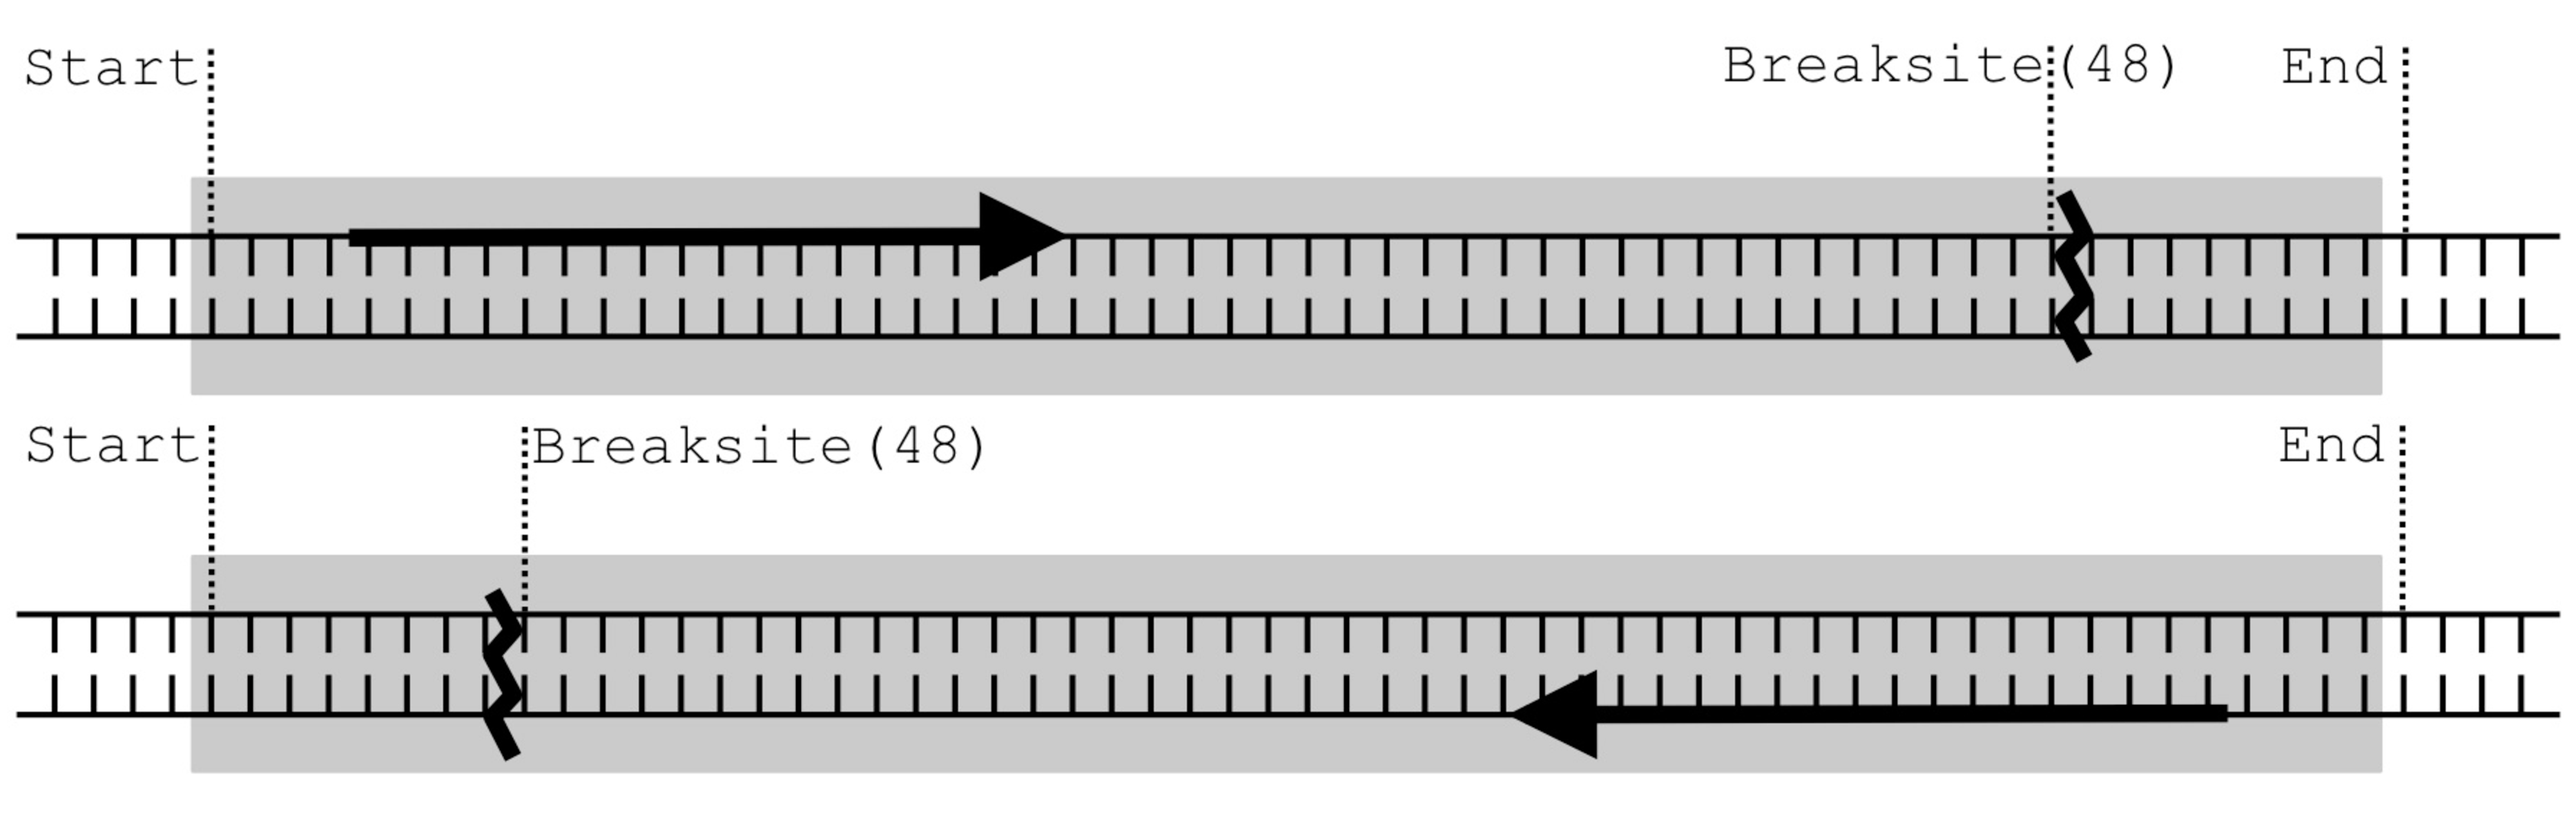
\includegraphics[width=\textwidth]{nonendogenous_breaksite}
\caption{\textbf{Non-endogenous breaksite} strategies are shown in the ``\texttt{+}'' strand orientation \textbf{(Top)} and ``\texttt{-}'' orientation \textbf{(Bottom)}. Diagrams are oriented so that chromosomal coordinates increase from left to right. The bold arrow represents the priming site and the jagged line represents the targeted nuclease site. The shaded area represents the non-endogenous cassette. The appropriate \texttt{Start} and \texttt{End} coordinates are marked. The \texttt{Breaksite} coordinate, 48 in this case, is determined with respect to the cassette sequence (\texttt{Breakseq}) in primer-to-target orientation.}
\label{overflow}
\end{figure}
\paragraph{} The annotation is more complicated for non-endogenous breaksite libraries than for endogenous breaksites because the pipeline requires extra information about the genomic location of the cassette as well as the cassette's sequence and targeted nuclease site. The \textbf{breaksite cassette} is treated very similarly to the breaksite locus of the endogenous breaksite library. The \texttt{Chr}, \texttt{Start}, \texttt{End}, and \texttt{Strand} fields together fully annotate the cassette position and orientation. The \texttt{Chr} field contains the name of the chromosome harboring the cassette. The \texttt{Strand} field is the orientation of the cassette in primer-to-target direction, either ``\texttt{+}'' or ``\texttt{-}''. Again, the pipeline follows the convention of requiring the start coordinate to be not greater than the end coordinate. Regardless of orientation, the \texttt{Start} field is the coordinate immediately following the last chromosomal coordinate before the breaksite cassette. The \texttt{End} field is the chromosomal coordinate of the first basepair after the end of the breaksite cassette (Fig. 2). \emph{Note: these coordinates refer to the unmodified reference chromosome, not the coordinates of the chromosome with cassette inserted. \texttt{Start} and \texttt{End} will be equal in the case that the cassette has been inserted with no loss of endogenous sequence.}
\paragraph{} With the position and orientation of the breaksite cassette fully annotated, all that is left to do is to specify the cassette sequence and annotate the breaksite locus within the cassette. The breaksite cassette sequence is given in the \texttt{Breakseq} field and should be the full cassette sequence written in the primer-to-target orientation. This is the case for both ``\texttt{+}'' and ``\texttt{-}'' orientations. The breaksite locus, as in endogenous breaksite libraries, is fully determined by the priming site and the targeted site. While in endogenous breaksite libraries the priming site must be given explicitly, this is not so in non-endogenous breaksite libraries because the pipeline will determine the location of the priming site by searching for the primer sequence within the breaksite sequence. However, that still leaves one last piece of information to be accounted for in the non-endogenous breaksite libraries and that is the specific location of the targeted site. The \texttt{Breaksite} field contains the last coordinate before the targeted site, with respect to the sequence entered in \texttt{Breakseq} (Fig. 2). This fully annotates the non-endogenous breaksite library.


\section{Sequence Information}
\textbf{MID, Primer, Adapter, Cutter}
\paragraph{} Each of these fields relay nucleotide sequences to the pipeline and may only contain the characters \texttt{A}, \texttt{C}, \texttt{G}, and \texttt{T}. Each should be written in the orientation that they would be sequenced on the first read of a paired-end sequencing run. The \texttt{MID} field may be blank if the library did not contain a multiplex identifier sequence ahead of the primer. These are the first expected bases on the first read of paired-end sequencing. The \texttt{Primer} field should contain the sequence of the priming site from the breaksite strategy and may not be blank. On the first read, these will be bases immediately following the MID. The \texttt{Adapter} field should contain the sequence of the adapter used to prepare the captured translocation sequences (frequently used is the AP2 adapter). Although the adapter will contain the first several bases on the second read of a paired-end sequencing, it should be submitted in the orientation that it would be found on the first read. Finally, the \texttt{Cutter} field should contain the target sequence of the frequent cutter enzyme used to fragment the DNA when creating the library. For libraries prepared using sonication, or a fragmentation technique other than with a frequent cutter enzyme, this field should be left blank. 



\section{Developer and Technical Notes}
\subsection*{Format}
\paragraph{} The metadata file is a tab-delimited plain text file that includes a header row, followed by a row for each library. Each row should be separated by the UNIX newline character. However, researchers will most frequently create/edit the metadata file using Microsoft Excel which, upon saving regular text files, writes the carriage-return character between rows in place of the newline character. Therefore, any processing must first replace these carriage-return characters, usually denoted ``\texttt{\textbackslash{}r}'', with the newline character, ``\texttt{\textbackslash{}n}''.
\paragraph{} The header row consists of the names of the columns each separated by a tab. There is no strict ordering of the columns and the column names are not case-sensitive. Future development of the pipeline, and downstream processing modules, must allow for flexibility with respect to these features.

\end{document}